\documentclass[a4paper,10pt]{article}
\usepackage{graphicx}
\usepackage{enumitem}
\usepackage{amsmath}
\usepackage{listings}
\usepackage[usenames,dvipsnames]{color}
\usepackage{bbm}
\usepackage{amsfonts}
\usepackage{hyperref}
\usepackage{multicol}
\usepackage{caption}
\usepackage{xcolor}
\hypersetup{
    colorlinks,
    linkcolor={red!50!black},
    citecolor={blue!50!black},
    urlcolor={blue!80!black}
}
\newcommand{\cfbox}[2]{%
    \colorlet{currentcolor}{.}%
    {\color{#1}%
    \fbox{\color{currentcolor}#2}}%
}
\usepackage[thinlines]{easytable}
\usepackage{url}
\usepackage{relsize}
\renewcommand*{\UrlFont}{\ttfamily\smaller\relax}
\newcommand\fnurl[2]{%
  \href{#1}{#2}\footnote{\url{#1}}%
}
%%%%%%%%%%%%%%%%%%%%%%%%%%%%%%%%%%%%%%%%%%%%%%%%%%%%%%%%%%%%%%%%%%%%%%%%%%%%%%%%%%%%%%%%%%%
% MATLAB code listing
%
% This is the color used for MATLAB comments below
\definecolor{MyDarkGreen}{rgb}{0.0,0.4,0.0}
 
% For faster processing, load Matlab syntax for listings
\lstloadlanguages{Matlab}%
\lstset{language=Matlab, % Use MATLAB
frame=single, % Single frame around code
basicstyle=\tiny\ttfamily, % Use small true type font
keywordstyle=[1]\color{Blue}\bfseries, % MATLAB functions bold and blue
keywordstyle=[2]\color{Purple}, % MATLAB function arguments purple
keywordstyle=[3]\color{Blue}\underbar, % User functions underlined and blue
identifierstyle=, % Nothing special about identifiers
% Comments small dark green courier
commentstyle=\usefont{T1}{pcr}{m}{sl}\color{MyDarkGreen}\small,
stringstyle=\color{Purple}, % Strings are purple
showstringspaces=false, % Don't put marks in string spaces
tabsize=5, % 5 spaces per tab
%
%%% Put standard MATLAB functions not included in the default
%%% language here
morekeywords={xlim,ylim,var,alpha,factorial,poissrnd,normpdf,normcdf},
%
%%% Put MATLAB function parameters here
morekeywords=[2]{on, off, interp},
%
%%% Put user defined functions here
morekeywords=[3]{FindESS, homework_example},
%
morecomment=[l][\color{Blue}]{...}, % Line continuation (...) like blue comment
numbers=left, % Line numbers on left
firstnumber=1, % Line numbers start with line 1
numberstyle=\tiny\color{Blue}, % Line numbers are blue
stepnumber=5 % Line numbers go in steps of 5
}

\usepackage{xspace}
\newcommand*{\eg}{e.g.\@\xspace}
\newcommand*{\ie}{i.e.\@\xspace}

\makeatletter
\newcommand*{\etc}{%
    \@ifnextchar{.}%
        {etc}%
        {etc.\@\xspace}%
}
\makeatother
%%%%%%%%%%%%%%%%%%%%%%%%%%%%%%%%%%%%%%%%%%%%%%%%%%%%%%%%%%%%%%%5

\newcommand\scalemath[2]{\scalebox{#1}{\mbox{\ensuremath{\displaystyle #2}}}}


%opening
\title{Automatic Applicator\\Requirement Specifications}
\author{Munzir Zafar}

\begin{document}

\maketitle

\section{Introduction}
This document lays out the specifications for the \emph{Automatic Applicator} being built to fulfill
the need of replacing human operator from the job of spray painting plastic parts in order to increase
safety, consistency, production throughput and reduce operation costs and wastages of the painitng process. 

\section{Environment}
The layout of the Paint shop at Port Qasim Plant of Auvitronics is as shown in figure \ref{fig:Layout}. The sequence of operations is: 
 Cleaning, Painting, Baking, Stacking in racks, Drying in racks for 24 hours, Quality Assurance,
 Reworking if needed and Packaging. A video clip giving a tour of the paint shop can be found \fnurl{https://drive.google.com/file/d/0B0hRGVYqXqmJWUFpQk9kdjBxNXM/view?usp=sharing}{here}.
 A similar layout is also present in the Hub Plant of Auvitronics and is shown in figure \ref{fig:Layout2}. Its video can be found \fnurl{https://drive.google.com/file/d/0B0hRGVYqXqmJbUg4R2wxZ3BZelU/view?usp=sharing}{here}.
 Marks A, B, C and D on the figures are the locations where human painters currently operate.
 Those are the locations at which the robot arm needs to be installed. A number of human operators are moving around these spots
 for the purpose of moving in the cleaned parts from the Cleaning area and taking out the painted parts from painting area to
 the baking area. So it is important that the machine is stable in response to any collisions from walking humans. Also, it
 should have hard safety limits so as to avoid any harm in case of machine error causing parts to go out of the operating zone.
 These limits should be present in the hardware and not just at the software level. Also, the machine should have protection 
 from paint particles. The temperature of the paintshop is maintained around $25^oC$.
\begin{figure}[h]
\centering \frame{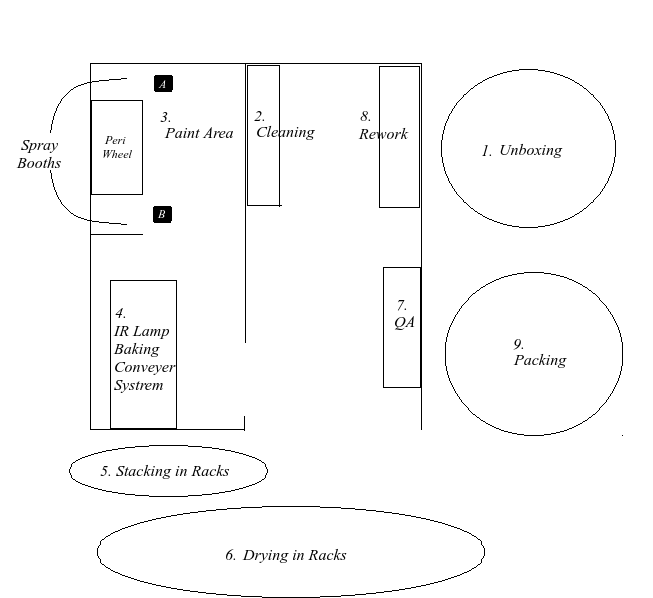
\includegraphics[width=0.8\columnwidth]{Figures/PaintShopLayout.png}}
\caption{A rough drawing of the existing layout of the paint shop at Port Qasim}
\label{fig:Layout} 
\end{figure}

\begin{figure}[h]
\centering \frame{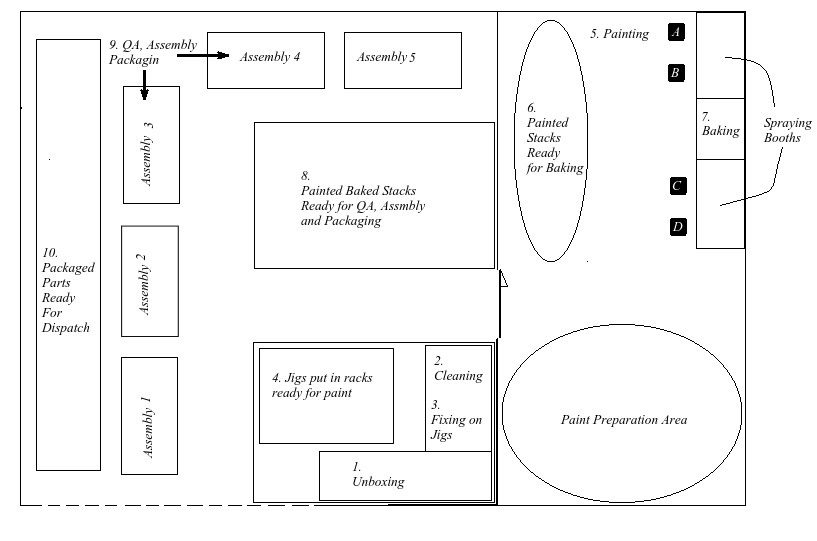
\includegraphics[width=0.8\columnwidth]{Figures/PaintShopLayout2.png}}
\caption{A rough drawing of the existing layout of the paint shop at Hub}
\label{fig:Layout2} 
\end{figure}


\section{Performance}
\subsection{Speed of Operation}
Current production throughput of one spraybooth is 400 jobs a day or 50 jobs an hour for the wheel cap. A similar rate is there
for all other parts where each job comprises of spray-painting one set arranged on a jig. The speed of horizontal motion
based on the maximum sizes of the jigs (5ft $\times$ 4ft) assuming full coverage will be attained by forty-eight $5$-feet lines separated
by one inch along the breadth. The required speed can be calculated as follows:
\begin{align}
 v_{max} &= \frac{\text{motion giving full coverage}}{\text{time per job}} \nonumber \\
 &= \frac{5\text{ ft } \times 48}{1 \text{ minute }} \nonumber \\
 &= \frac{240\text{ ft}}{60 \text{ sec}} \nonumber \\
 &= 4 ft/s \nonumber \\
 &= 1.2 m/s 
\end{align}


\subsection{Spraying Gun Paths and Contours}
 The parts being painted currently are shown in figure \ref{fig:Parts}. Apart from the wheel-cap all parts are painted in sets
 arranged in the form of an array fixed on a jig. Figure \ref{fig:Jigs} shows two such jigs. It is important for the purpose
 of the design to know what the sizes of these jigs are and how many pieces are present in the set of each of these parts
 when arranged on the jig before painting. Table \ref{table:PartsAndJigs} shows the names of these parts numbered according 
 to the labels present in figure \ref{fig:Parts} along with the sizes of the Jigs and the count of parts per set.
 A video showing the human operator painting a robot can be found \fnurl{https://drive.google.com/file/d/0B0hRGVYqXqmJWnU3NXE0R1hPODA/view?usp=sharing}{here}.
\begin{figure}[ht!]
\centering \frame{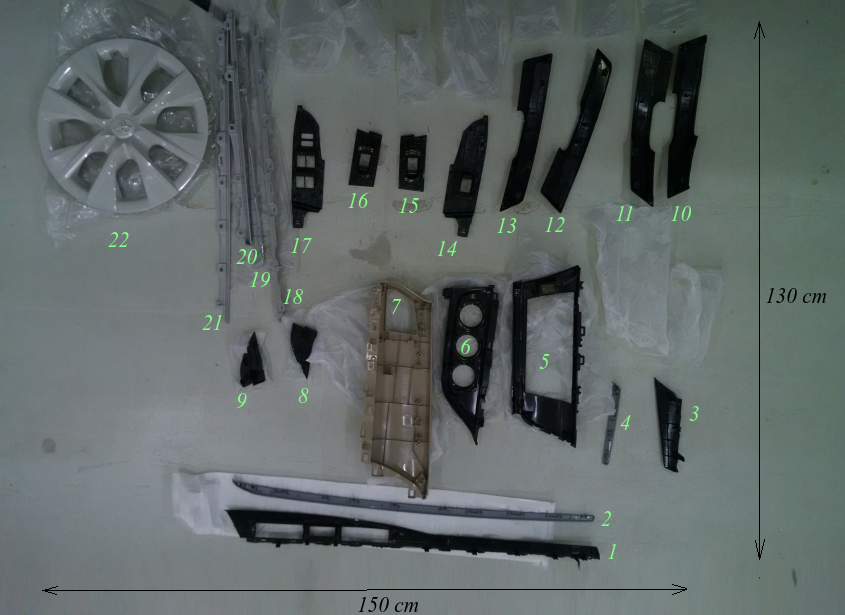
\includegraphics[width=0.6\columnwidth]{Figures/Parts.png}}
\captionsetup{singlelinecheck=off}
\caption[parts]{A snapshot of the collection of parts being painted currently}
\label{fig:Parts} 
\end{figure}

\begin{figure}[ht!]
\centering \frame{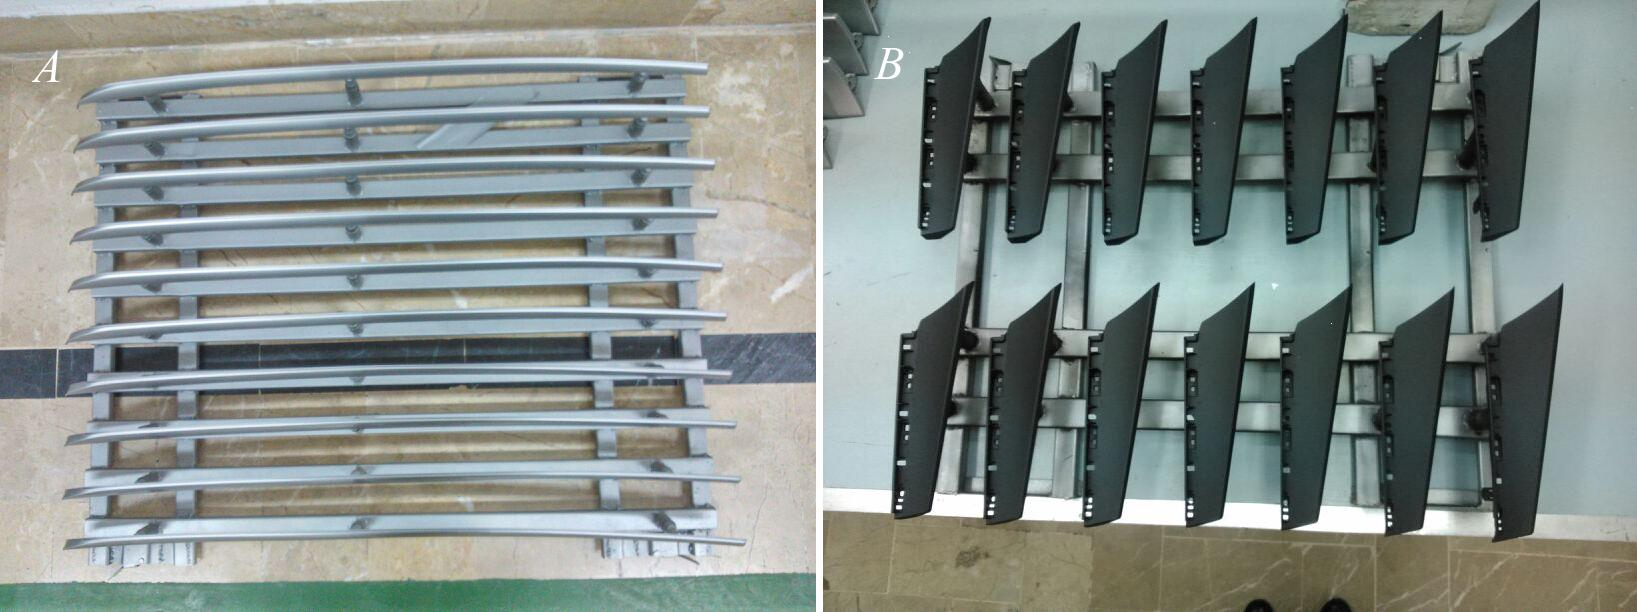
\includegraphics[width=\columnwidth]{Figures/Jigs.png}}
\captionsetup{singlelinecheck=off}
\caption[jigs]{A. Jig for part no. 18---Cover FR Door Trim RH B. Jig for part no. 3---Garnish S/A Inst Panel}
\label{fig:Jigs} 
\end{figure}

\begin{table}[ht!]
  \small
  \resizebox{\columnwidth}{!}{
    \begin{tabular}{|c|l|c|c|}
    \hline
    \textbf{S.No.} & \textbf{Part Name} & \textbf{Jig Size} & \textbf{Set Size} \\
      \hline \hline
    1 & Garnish S/A Instr. Panel & 3 ft $\times$ 19 in & 5 \\
    2 & Panel, Instr. CSTR Fin., CTR LWR & 3 ft $\times$ 14 in & 5 \\
    3 & Garnish S/A Inst Panel & 2 ft $\times$ 19 in & 14 \\
    4 & Panel Inst Lwr LH & 2 ft $\times$ 20 in & 20 \\
    5 & Panel S/A Instrument Cluster Finish (BLACK PIANO) & 2 ft $\times$ 22 in & 3  \\
    6 & Panel S/A Instrument Cluster Finish LWR CTR & 2 ft $\times$ 20 in &  4 \\
    7 & Garnish Assy, Instrument Cluster Finish Panel & 2 ft $\times$ 2ft & 3 \\
    8 & Panel RR Door Armrest Base, UPR LH & 2 ft $\times$ 20 in & 18 \\
    9 & Panel RR Door Armrest Base, UPR LHR & 2 ft $\times$ 20 in & 18 \\
    10 & Cover Door Assist Grip, RH & 2 ft $\times$ 20 in & 6 \\
    11 & Cover Door Assist Grip, LH & 2 ft $\times$ 20 in & 6 \\
    12 & Cover Door Assist Grip, RH (low) & 2 ft $\times$ 20 in & 6 \\
    13 & Cover Door Assist Grip, LH (low) & 2 ft $\times$ 20 in & 6 \\
    14 & Switch Set Power Window LH & 2 ft $\times$ 20 in & 10 \\
    15 & Switch Set Power Window RH & 2 ft $\times$ 20 in & 20 \\
    16 & Switch Set Power Window LH & 2 ft $\times$ 20 in & 20 \\
    17 & Switch Set Power Window Master LH & 2 ft $\times$ 20 in & 10 \\
    18 & Cover FR Door Trim RH & 2 ft $\times$ 20 in & 10 \\
    19 & Cover FR Door Trim, LH & 29 in $\times$ 22 in & 10  \\
    20 & Cover RR Door Trim, RH & 29 in $\times$ 22 in & 10 \\
    21 & Cover RR Door Trim, LH & 29 in $\times$ 22 in & 10 \\
    22 & Wheel Cap (Radius: 16 in) & N/A & 1 \\ \hline
      \end{tabular}
      }
\caption{Parts Being Painted along with Jig Sizes and Part Count per Set}
\label{table:PartsAndJigs}
\end{table}


\normalsize
\subsection{Programming}
The machine should have the ability to be programmed easily as parts are changed. It should have the ability to remember the planned
paths programmed with regards to each new part. Its memory should be scaleable and should be able to accomodate any number or type of
parts.
\subsection{Reach and Precision}  
The sizes of parts and jigs on which the arm will operate shown in table \ref{table:PartsAndJigs} indicate that the maximum length
of the jig is $3$ ft and the maximum width is $2$ ft. Adding one foot on either side for tolerance, we say the total coverage 
on the horizontal plane (say $XY$-plane) should be $5$ ft $\times$ $4$ ft (figure \ref{fig:Reach}). In addition to this, the spray gun should be able
to rotate about the $X$-axis and the $Y$-axis. This is important in order to allow the spray to access tilted surfaces on 
the inside of the parts. Since most parts also have near-vertical surfaces, only allowing for the afore-mentioned rotations will not
be enough, so we need the end-effector to be able to move vertically (that is, along the $Z$-axis), such that the spray direction
can be made perpendicular to such vertical surfaces on the side of a part. Since the parts are no more than $5$ inches long along the $Z$-dimension
and the spray should be $6$--$8$ inches away from the surface, the vertical range should be $1ft+5in+8in+1ft=3ft 1in$ where a one-foot tolerance is added to either side. Also, the
range of rotation about the $X$ and $Y$ axes should be $\pm 90^o$ when $0^o$ indicates the orientation where the spray direction
is along the $Z$-axis.
\begin{figure}[ht!]
\centering \frame{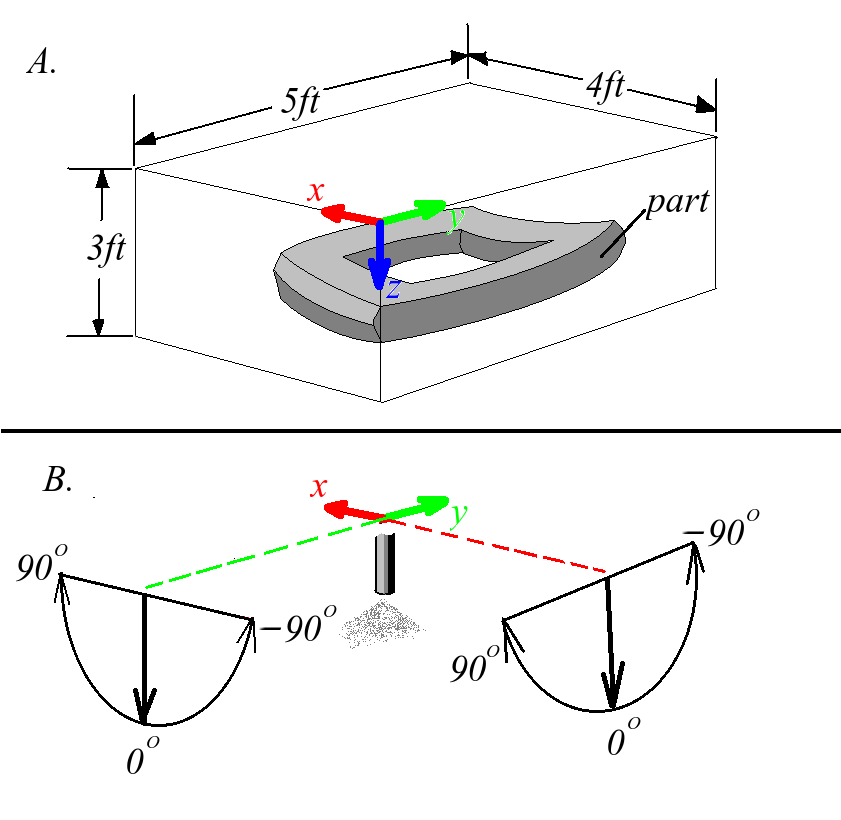
\includegraphics[width=0.8\columnwidth]{Figures/Reach.png}}
\captionsetup{singlelinecheck=off}
\caption[jigs]{A. Specification for End-effector Position Reach B. Specification for End-Effector Orientation Reach}
\label{fig:Reach} 
\end{figure}
Current wastage of the paint is significant owing to the fixed fluid flow and spread from the spray-gun. If 
the spread is made narrower wherever needed, wastage can be minimized. This also means that the control of position and orientation
of the end-effector should be precise. Better precision will result in minimization of this waste. The precision of control or
repeatability offered by other robot manufacturers (such as \fnurl{http://www.motoman.com/datasheets/Robot\%20Series\%20Brochure.pdf}{Motoman}, 
\fnurl{https://www.robots.com/kuka/kr-100-ha}{KUKA} and \fnurl{http://www.staubli.com/en/robotics/6-axis-scara-industrial-robot/specialized-robot/painting-robot/rx90-paint/}{Staubli}) 
ranges from $\pm 0.02mm$ to $\pm 0.5mm$. So, the precision of the designed robot should at least be better than $\pm 0.5mm$.

\subsection{Spraying Gun}
The spray gun has three adjustible parameters: \emph{Volume}, \emph{speed} and \emph{spread}. Increasing the \emph{volume}
 will increase the quantity of the spray coming out of the gun. Increasing the \emph{speed} will increase the
 speed with which the paint comes out of the gun. And increasing the \emph{spread} will increase the width of
 the flow coming out of the gun. The path plan being fed to the applicator when it is being programmed
 to spray a new part should provide the user the ability to program these three parameters along 
 the way. \emph{DevilBiss Compact} spray guns are currently in use. A video showing this gun can be found 
 \fnurl{https://drive.google.com/file/d/0B0hRGVYqXqmJWnU3NXE0R1hPODA/view?usp=sharing}{here}.

\section{Physical Size and Weight}
Based on the layout of the plant the footprint of the machine should be limited to $2$ft $\times$ $2$ft. There is no specific limit on 
the weight of the machine. 

\section{Power}
The power input to the machine is the standard three phase voltage with 400 / 230V on each phase.
Assuming power consumption is the only running cost of the machine, the limit on the wattage of the machine
will be determined from the current running cost of human painting. The idea is that the running cost of the 
machine shouldn't exceed the running cost of human painting. The monthly wages $H$ of the human operator is currently:
\begin{align}
 H &= \text{Rs. }22,000 \text{ per month} 
\end{align}
In order to find out the hourly expense $h$ of a human operatoror we divide it by the number of work-days in 
a month and number of work hours every day:
\begin{align}
 h &= \frac{\text{Rs. }22,000\text{/month}}{26 \text{workdays/month} \times 8 \text{work-hours/day}} \nonumber \\
 &= \text{Rs.} 105 \text{/hour}
\end{align}
The current electicity charges are Rs. 18 per kiloWatt-hour, so we conclude that the upper-limit $P_{max}$ of the 
power consumption is:
\begin{align}
 P_{max} &= \frac{\text{Rs. }105/h}{\text{Rs. }18/kWh} \nonumber \\
 &=5.83 kW
\end{align}
Such a power consumption will result in the same operation cost as a human operator. 
Of course, the actual consumption should be much lower than this to financially justify replacement of a human
operator with a machine and to recover the purchase cost of the machine well before its life ends.

% \section{Life}
% The machine should continue to operate for at least \cfbox{red}{????} years without problems and minimum maintenance expenses.
% 
% \section{Cost}
% This limit is determined based on the knowledge from the market 
% of similar machines that can be imported to Pakistan. The \cfbox{red}{machine} ???? from ???? \cfbox{red}{company} is \cfbox{red}{priced} at Rs. ??? and after adding
% the \cfbox{red}{import duties} this cost reaches up to Rs. ?????. So the total production cost should, by no means, exceed this cost and at least be
% aimed at half of this price.

\section{Life and Cost Specification}
Say, $L$ is the number of months in which we want the investment of the buyer to fully recover. And say $P$ (kW) is the operating power consumed by the machine then
the monthly savings $S$ will be:
\begin{align}
 S &= \frac{P_{max}-P}{P_{max}} \times H \nonumber \\
 &= \left(1-\frac{P}{P_{max}}\right)H 
\end{align}
Then the price $p$ at which the buyer purchased this machine is:
\begin{align}
 p &= SL \nonumber \\
 &= \left(1-\frac{P}{P_{max}}\right)HL 
\end{align}
Working on designing such a machine is financially feasible for the company if the overall revenue generated by the machine as a result of this 
project exceed the overall costs. If the cost of production of one machine is $C_p$, the design cost is $C_d$ and the estimated number of pieces 
we will sell is $n$ then:
\begin{align}
 C_p + \frac{C_d}{n} &< p \nonumber \\
 C_p + \frac{C_d}{n} &< \left(1-\frac{P}{P_{max}}\right)HL \label{CostSpec}
\end{align}

The relationship \ref{CostSpec} is the specification for the power consumption, useful life of the machine, production cost of the machine
and design cost of the machine. If the inequality is satisfied by a good enough margine, then the project is satisfying our specifications.
As an example, if the life of the machine $L=60$ months, power consumption $P=1kW$, number of pieces we will put to use or sell are $n=15$,
design cost is $C_d = \text{Rs.}800,0000$ then the production cost should stay well below $\left(1-\frac{P}{P_{max}}\right)HL-\frac{C_d}{n}$
$=\left(1-\frac{1kW}{5.83kW}\right) \times \text{Rs.}22,000 \times 60-\frac{\text{Rs.}800,000}{15}$ $=\text{Rs.}10,40,286$

\section{Conclusion}
The purpose of this document was to lay out the specifications that need to be satisfied in order for the project to be deemed as
satisfactory, successfully meeting the goals we laid out in the \emph{Statement of Need}. We specified in the preceding paragraphs the
environment, the requirements on speed, reach, precision, spraying, power, life, cost and size of the machine. This 
document should serve as the basis on which design decisions for the project are taken.

% \newpage
% Based on this the size of the machine should be 
%  limited to ?????????
% \begin{itemize}
% \normalsize
%  \item The paint to be applied on the wheel-cap is a mixture of three compponents purchased from Japan: 
%   Recrack470, Recrack-Thinner-5739 and Recrack470-Hardener. The paint being applied on other parts are 
%   ?????
%  \item The spray gun has three adjustible parameters: \emph{Volume}, \emph{speed} and \emph{spread}. Increasing the \emph{volume}
%  will increase the quantity of the spray coming out of the gun. Increasing the \emph{speed} will increase the
%  speed with which the paint comes out of the gun. And increasing the \emph{spread} will increase the width of
%  the flow coming out of the gun. The path plan being fed to the applicator when it is being programmed
%  to spray a new part should provide the user the ability to program these three parameters along 
%  the way.
%  \item The power input to the machine is the standard three phase voltage with 220V on each phase.
%  \item The layout of the Paint shop at Port Qasim is as shown in figure \ref{fig:Layout}. The sequence of operations is: 
%  Unboxing, Cleaning, Painting, Baking, Stacking in racks, Drying in racks for 24 hours, Quality Assurance,
%  Reworking if needed and Packaging. Marks A and B on the figure are the locations where human painters currently operate.
%  Those are the locations at which the robot arm needs to be installed. Based on this the size of the machine should be 
%  limited to ?????????
% \normalsize
% \begin{figure}[h]
% \centering \frame{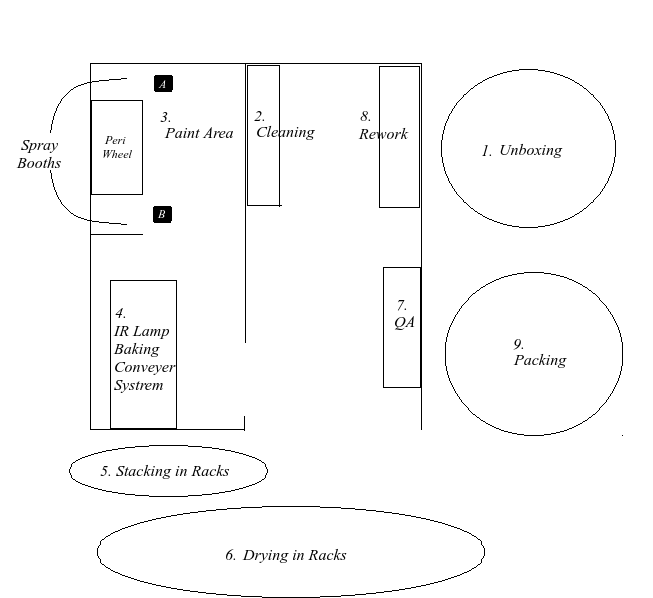
\includegraphics[width=0.6\columnwidth]{Figures/PaintShopLayout.png}}
% \caption{A rough drawing of the existing layout of the paint shop}
% \label{fig:Layout} 
% \end{figure}
%  \item Current running cost for the painting process is Rs. ?????. So the operating expenses of the machine should not
%  exceed this limit.
%  \item Current wastage of the paint is ?????. The machine should ideally reduce this wastage.
%  \item Current production throughput of one spraybooth is 400 jobs a day or 50 jobs an hour. The machine should at least
%  match these requirements or exceed it. Based on this the speed of the end effector is determined to be ??????
%  \item The new machine should operate for at least 5 years without problems.
%  \item The total production cost for the machine should not exceed Rs. ?????
%  \item The parts being painted currently are shown in the figure \ref{fig:Parts}. Their names are:
% \begin{figure}[h]
% \centering \frame{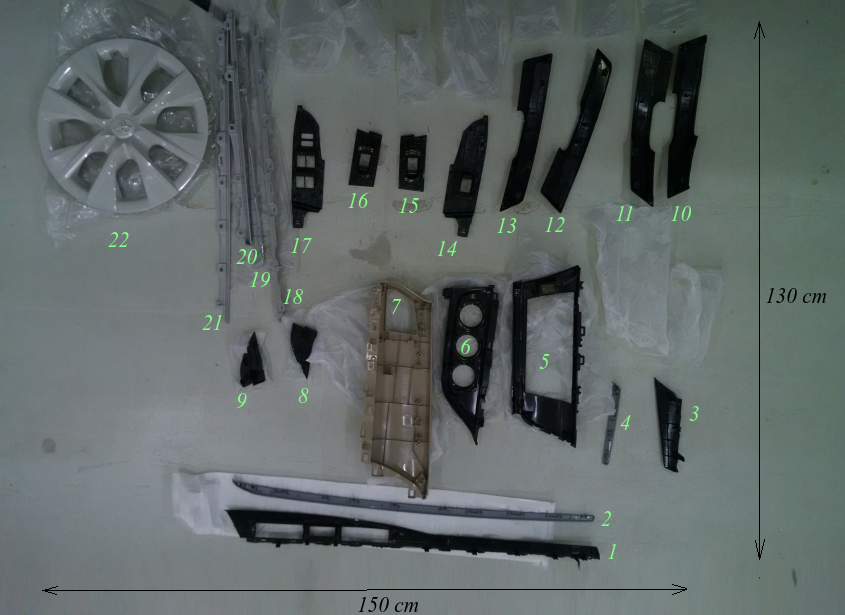
\includegraphics[width=0.6\columnwidth]{Figures/Parts.png}}
% \captionsetup{singlelinecheck=off}
% \caption[parts]{A snapshot of the collection of parts being painted currently}
% \label{fig:Parts} 
% \end{figure}
%    \tiny{
%   \begin{multicols}{4}
%   \begin{enumerate} 
%     \item Garnish S/A Instr. Panel 
%     \item Panel, Instr. CSTR Fin., CTR LWR 
%     \item Garnish S/A Inst Panel 
%     \item Panel Inst Lwr LH 
%     \item Panel S/A Instrument Cluster Finish (BLACK PIANO) 
%     \item Panel S/A Instrument Cluster Finish LWR CTR 
%     \item Garnish Assy, Instrument Cluster Finish Panel
%     \item Panel RR Door Armrest Base, UPR LH 
%     \item Panel RR Door Armrest Base, UPR LHR 
%     \item Cover Door Assist Grip, RH 
%     \item Cover Door Assist Grip, LH 
%     \item Cover Door Assist Grip, RH (low) 
%     \item Cover Door Assist Grip, LH (low) 
%     \item Swith Set Power Window LH 
%     \item Switch Set Power Window RH 
%     \item Swith Set Power Window LH 
%     \item Switch Set Power Window Master LH
%     \item Cover FR Door Trim RH 
%     \item Cover FR Door Trim, LH 
%     \item Cover RR Door Trim, RH 
%     \item Cover RR Door Trim, LH 
%     \item Wheel Cap
%   \end{enumerate}
%   \end{multicols}
%   }
%   Based on the dimensions of these parts the reach of the robot arms is determined as follows: ??????  And the required precision turns out to be ?????
% \end{itemize}
% 


% The gun being used 
% 
% \section{Which paint is being applied?}
% Ask Irfan
% 
% \section{What is the layer thickness of the paint being applied?}
% Ask Irfan
% 
% \section{What are the parts on which paint is being applied?}
% Get photo from Faisal
% 
% \section{Where is the applicator going to be installed? Layout of the plant?}
% Ask Irfan
% 
% \section{Power input voltage?}
% 220V, Confirm from Irfan
% 
% \section{Current running cost that is targetted to be minimized?}
% Ask Irfan
% 
% \section{Current waste that is targetted to be minimized?}
% Ask Irfan
% 
% \section{Current production throughput that we aim to maintain or increase?}
% Ask Irfan
% 
% \section{How many years should the applicator continue to serve?}
% Ask Muhammad Ali
% 
% \section{Cost of finished product? What are the competitors offering that we want to compete with?}
% Do your research! 
\newpage
\section{List of Companies who Provide Painting Robots}
\tiny
\begin{multicols}{4}
\begin{enumerate}
  \item \fnurl{http://www.motoman.com/products/robots/painting-robots.php}{YASKAWA}---US
  \item \fnurl{http://www.compass-automation.com/}{Compass Automation}---US
  \item \fnurl{http://www.irbs.us/implementacion.php}{irbs}---US
  \item \fnurl{http://www.kuka-robotics.com/en/solutions/branches/automotive/start.htm}{KUKA}---Germany
  \item \fnurl{http://www.smr-automotive.com/painting.html}{SMR}---Germany
  \item \fnurl{http://robot.fanucamerica.com/Products/Robots/painting-robots.aspx}{FANUC America}---Japan
  \item \fnurl{http://www.abb.com/References/Default.aspx?db=db/db0003/db001466.nsf&c=388F798560C0E2AAC1257559003B752B}{ABB China}---China
  \item \fnurl{http://www.alibaba.com/product-detail/Robot-Paint-Shop-for-Automotive-Parts_557884730.html}{Alibaba Automatic Paint shops}, \fnurl{http://www.honglichang.co.in/robotic-painting-line-for-automobile-parts-2539502.html}{Honglichang}, \fnurl{http://www.tradeindia.com/selloffer/4518892/Robot-Paint-Shop-For-Automotive-Parts.html}{TradeIndia}---China
  \item \fnurl{http://www.staubli.com/en/robotics/robot-solution-application/painting-robot/}{Staubli}---Switzerland
  \item \fnurl{http://www.epistoliorobot.com/en/}{Epistolio}---Italy
  \item \fnurl{http://gse-m.com/products/sfs/}{Surface Finishing Systems}---Malaysia
  \item -\fnurl{http://www.durr.com/fileadmin/user_upload/Erlebniswelt/Innovations/DURR_EcopaintRobot_EN.pdf}{Ecopaint}---US
  \item -\fnurl{http://www.eisenmann.com/en/products-and-services/general-finishing/paint-shops-for-plastic-parts/paint-systems.html}{Eisenmann}---Germany
  \item -\fnurl{https://robotics.kawasaki.com/en/applications/robotic-painting/}{Kawasaki}---Japan
  \item -\fnurl{http://www.doolim-robotics.com/source/images/img/media/Doolim_cat2015_Coating_e.pdf?ckattempt=1}{Doolim}---Korea
  \item -\fnurl{http://www.abbaustralia.com.au/cawp/seitp202/c821f1979f2a2ba3c1257ecd001ca713.aspx}{ABB Australia}---Switzerland
  \item -\fnurl{http://paintboxuk.com/paint-application}{Paintbox}---UK
  \item --\fnurl{http://www.intechpower.com/products/cast-parts-for-electrically-insulated-robotic-arm}{INTECH Power-core}
  \item --\fnurl{http://www.turbospray.com/finishing-systems-2/}{Turbo Spray} 
  \item ---\fnurl{http://www.isravision.com/AUTOMOTIVE------_site.site..html_dir._nav.193_likecms.html}{ISRA Vision} 
  \item ----\fnurl{http://www.benet-automotive.cz/en/production/paint-shop}{Benet Automotive} 
\end{enumerate}
\end{multicols}
\section{Other possible specifications?}
Do your research! \\
\begin{multicols}{2}
\begin{enumerate}
  \item \fnurl{http://www.robotics.org/content-detail.cfm/Industrial-Robotics-Industry-Insights/The-Art-of-Industrial-Painting-with-Robots/content_id/4447}{The Art of Industrial Painting with Robots} 
  \item \fnurl{http://www.pfonline.com/articles/applying-robotics-to-your-paint-line}{Applying Robotics to your Paint Line} 
  \item \fnurl{www.ifr.org/index.php?id=59&df=Progress_in_robotic_painting_systems.doc}{Progress in Robotic Painting Systems} 
  \item \fnurl{http://www.automotivemanufacturingsolutions.com/process-materials/a-new-generation-for-paint-robots}{A New Generation for Paint Robots} 
  \item \fnurl{http://issinstitute.org.au/wp-content/media/2011/04/ISS-FEL-REPORT-C-KELLY-low-res.pdf}{Automotive Painting Technology into the 21st Century} 
  \item -\fnurl{http://www.roboticsbible.com/spray-painting-robot.html}{Robotics Bible} 
\end{enumerate}
\end{multicols}
% \section{Introduction}
% \section{Environment}
% \section{Performance}
% \section{Physical Size and Weight}
% \section{Power}
% \section{Life}
% \section{Reliability}
% \section{Cost}
% \section{Manufacturing Process}
% \section{Maintenance}

\end{document}
